% #############################################################################
% This is Chapter 4
% !TEX root = ../main.tex
% #############################################################################
% Change the Name of the Chapter i the following line
\fancychapter{Speed Dating}
\cleardoublepage
% The following line allows to ref this chapter
\label{chap:implement}

Speed Dating is a design method for rapidly exploring application concepts, their interactions, and contextual dimensions, requiring no technology implementation. It was developed at Carnegie Mellon University for accessing finer-grained insights into user needs, and identifying critical contextual dimensions for the design space ~\cite{Davidoff2007}. The main drive for developing such methodology was the lack of availability of methods that help design teams transition from ideation to iteration. Moreover, the authors state that, in ubiquitous computing, important design and contextual risk factors are not discovered before the deployment of a system, which can have a significant negative impact on the course or viability of a given project.

Aiming at solving these issues, speed dating supports low-cost rapid comparison of design opportunities and situated applications by creating structured, bounded, serial engagements. In addition, it helps teams contextualize multiple implementations, as well as critical aspects of individual applications, quickly foregrounding potential precarious issues before any implementation. It tests the researcher's initial ideas of problem definition and scope against user needs and the contextual factors that underlie them, while minimizing costs and time demands. Speed dating enables the researcher to explore the outermost frontiers of the design space, "presenting users with scenarios that push social boundaries to uncover where these boundaries actually lie” ~\cite{Davidoff2007}.

This method consists of a two-stage process, settling between sketching and prototyping. The first stage, named 'need validation', involves the use of personas, scenarios, and storyboards in a process aimed at exposing and validating user needs. The second stage, labeled 'user enactments', combines experience prototyping strategies and key concepts from the speed dating method within the elicitation of a second round of feedback pointed at finding a more full run of conceivable outcomes for the design.

We chose to apply the speed dating methodology since it allowed us to get a deeper understanding of our users' needs, while at the same time increasing our design effectiveness and efficiency. This approach was essential in exploring the complex set of factors, contextual dimensions, and design considerations that characterize a diverse and ambitious project such as this one. In the following subsections, we describe the work we have conducted in each of the stages of this methodology.

\section{Need validation}

The need validation stage of speed dating consists of presenting a set of storyboards to a group of target users, to synchronize the design opportunities researchers found with the needs users perceive. These storyboards help designers prioritize user demands, map areas for innovation more clearly, and use that focus to narrow the design space for implied implementations. ~\cite{Davidoff2007}

The first step of this phase is to focus concepts on user needs, where teams generate and cluster concepts around the needs identified in the conducted research. ~\cite{Davidoff2007} This is achieved by creating a collection of personas and scenarios that fall on both sides of boundaries the design team has speculated on. 

\begin{figure}[!h]
    \centering
    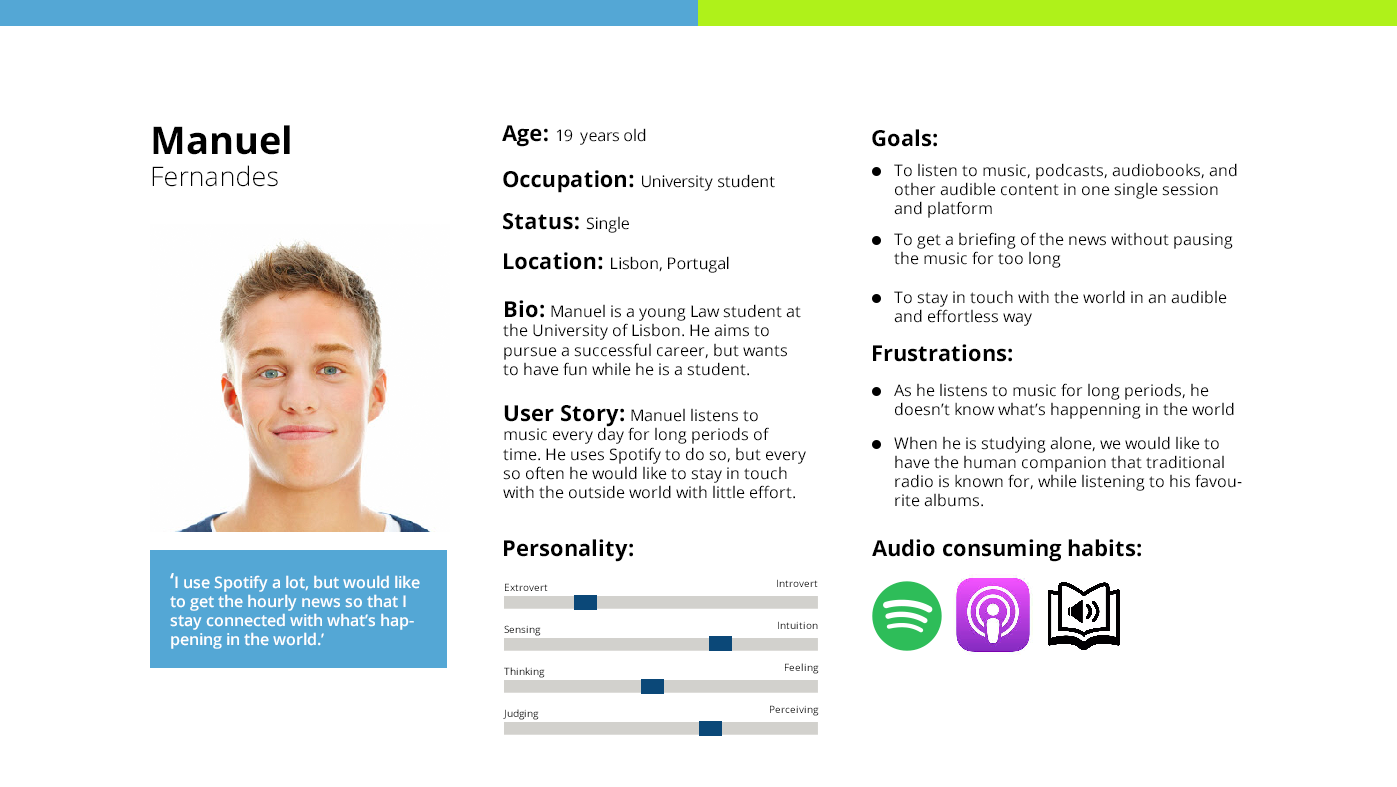
\includegraphics[width=\columnwidth]{./Images/persona.png}
    \caption{Example of one of the created personas.}
    \label{fig:persona}
\end{figure}

To do so, we have produced a set of four personas, based on four different potential users of this solution. To make them feel as real as possible, each persona was attributed an age, occupation, status, location, biography, user story, goals, frustrations, personality traits, and audio media consuming habits. The latter attribute is the main characteristic that differentiates the created personas from each other, so that we can understand if the portrayed functionalities of this platform would appeal to all ranges of potential users, even those that don't have very substantial audio listening habits on their routines. A summary of each persona is presented in the following list:

\begin{itemize}
	\item Manuel Fernandes, a university student that is a power-user of Spotify, who feels 'disconnected' from the world while indulging in all-day music listening sessions using the on-demand service;
	\item Carolina Santos, a software engineer that enjoys the interactivity of traditional terrestrial radio stations, but also enjoys the on-demand selection of her favorite songs that a music streaming service provides;
	\item Rita Silva, a middle-aged school teacher whose audio listening habits consist of a few minutes per day, tuning into her favorite radio station to listen to the news;
	\item Tomás Ventura, a truck driver that relies heavily on radio stations for his entertainment, but is getting tired of the repetitive music choice.
\end{itemize}


A subsequent set of scenarios was attributed to each of these four personas. Each scenario represents a distinct use case of this platform, focusing on situations where it is easy for participants to imagine themselves performing the mentioned activities.

We have represented these personas and their respective scenarios in a set of storyboards that document how each need arises in daily life, and how the concept intervenes to improve the quality of life. To develop such materials, we have begun by using the traditional sketching method by drawing these storyboards on paper.

\begin{figure}[!h]
    \centering
    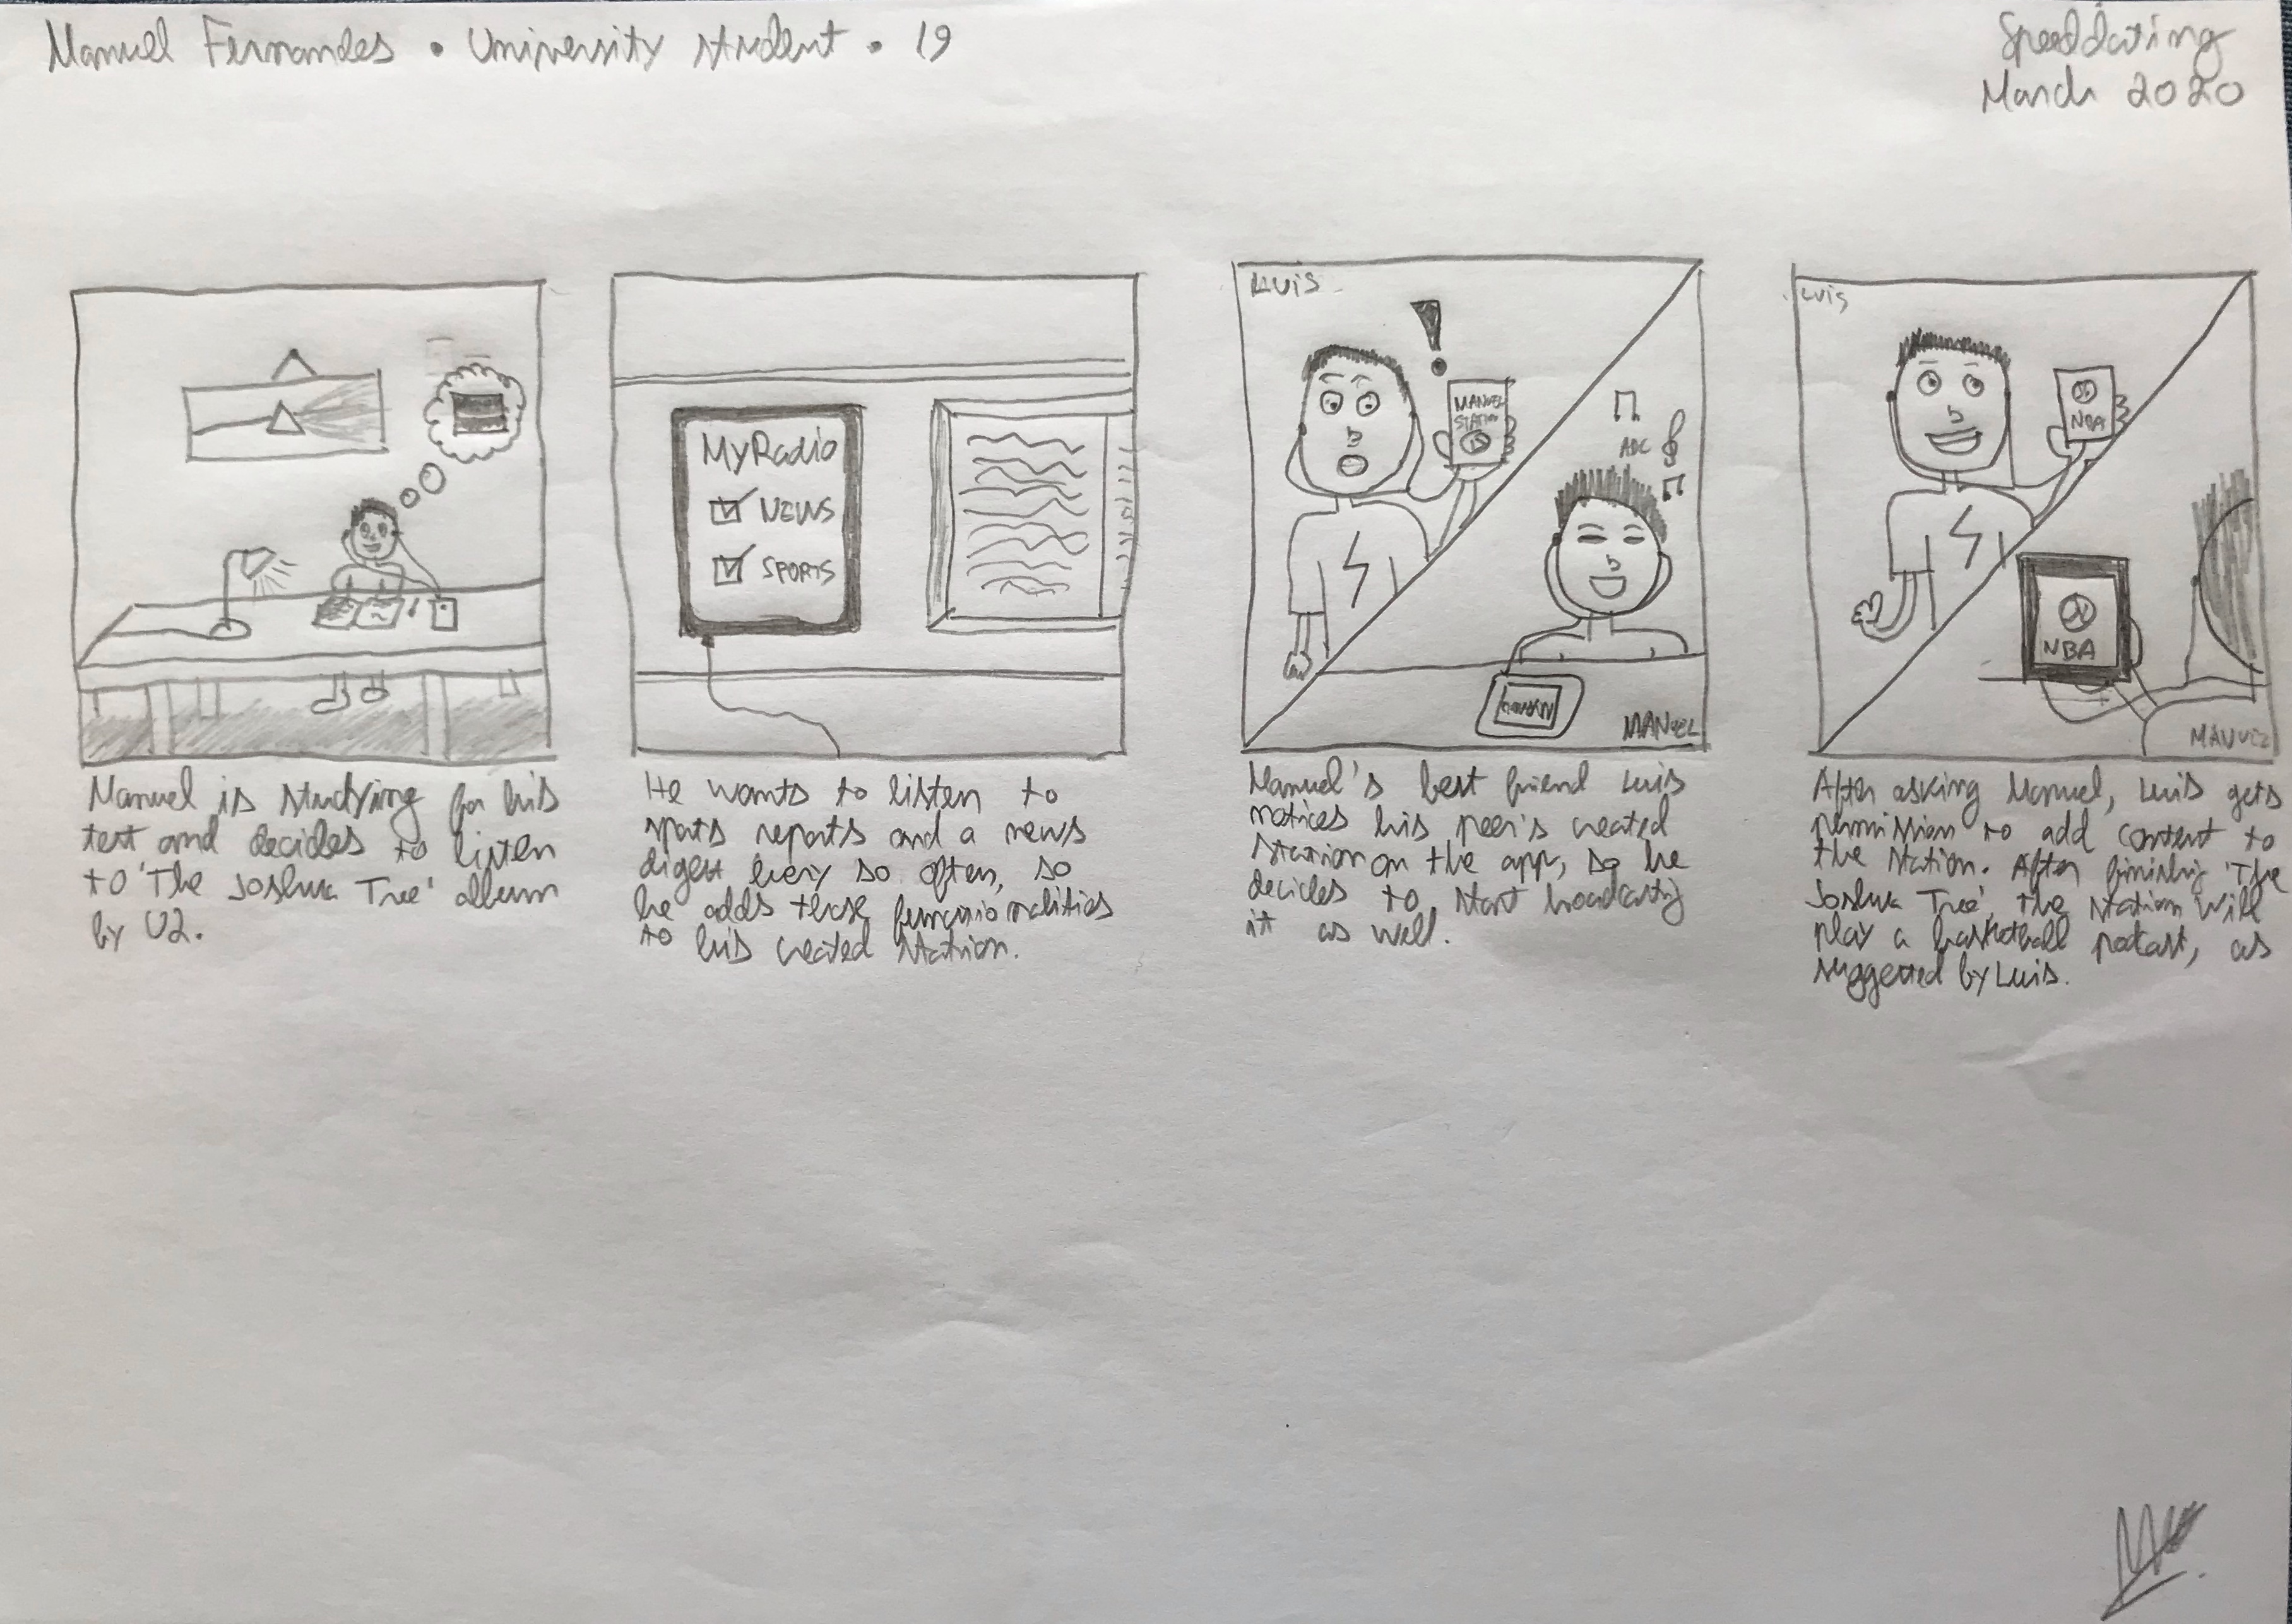
\includegraphics[width=\columnwidth]{./Images/storyboard.jpg}
    \caption{Example of one of the created storyboards, with the 'Manuel Fernandes' persona.}
    \label{fig:storyboard}
\end{figure}

The next step was to conduct a session where we presented this set of storyboards to small groups of target users. The original guidelines of the speed dating methodology state that these sessions should happen in a physical location; yet, as our study was conducted amid the 2020 COVID-19 pandemic, we had to circumvent this challenge, to comply with social distancing measures imposed by our country. Thus, we have conducted a total of five remote sessions, via the Google Meet platform: three of them with users ranging from 18 to 24 years old; one with ages ranging from 25 to 35 years old; and a final session with ages ranging from 35 to 55 years old. The participating users are reported in table ~\ref{tab:users}. The duration of each session ranged from 30 to 45 minutes. The audio of the session was recorded with the consent of all participating users, in order to facilitate the note-taking and analyzing processes. A consent form was digitally signed by all participating users.

{\renewcommand{\arraystretch}{1.35}%
\begin{table}[]
\centering
\begin{tabular}{|c|c|c|c|c|}
\hline
\multirow{2}{*}{\textbf{Age}} & \multicolumn{2}{c|}{\textbf{Preliminary User Research}} & \multicolumn{2}{c|}{\textbf{Speed Dating}}          \\ \cline{2-5} 
                              & \textbf{Diary Study}        & \textbf{Interview}        & \textbf{Need Validation} & \textbf{User Enactments} \\ \hline
18 & \checkmark & \checkmark & \checkmark & \checkmark \\ \hline
18 &   &   & \checkmark & \checkmark \\ \hline
18 &   &   & \checkmark & \checkmark \\ \hline
19 &   &   &   & \checkmark \\ \hline
19 &   &   & \checkmark & \checkmark \\ \hline
20 &   &   & \checkmark & \checkmark \\ \hline
21 & \checkmark & \checkmark &   &   \\ \hline
22 & \checkmark & \checkmark & \checkmark & \checkmark \\ \hline
22 & \checkmark & \checkmark & \checkmark & \checkmark \\ \hline
22 & \checkmark & \checkmark &   &   \\ \hline
22 & \checkmark & \checkmark &   &   \\ \hline
22 & \checkmark & \checkmark &   &   \\ \hline
22 & \checkmark & \checkmark &   &   \\ \hline
22 &   &   & \checkmark & \checkmark \\ \hline
22 &   &   & \checkmark & \checkmark \\ \hline
22 &   &   & \checkmark & \checkmark \\ \hline
22 &   &   & \checkmark & \checkmark \\ \hline
22 &   &   &   & \checkmark \\ \hline
22 &   &   &   & \checkmark \\ \hline
24 &   &   & \checkmark & \checkmark \\ \hline
27 & \checkmark & \checkmark &   &   \\ \hline
32 &   &   &   & \checkmark \\ \hline
33 &   &   &   & \checkmark \\ \hline
36 &   &   & \checkmark & \checkmark \\ \hline
38 &   &   &   & \checkmark \\ \hline
43 &   &   & \checkmark & \checkmark \\ \hline
43 &   &   & \checkmark & \checkmark \\ \hline
46 &   &   &   & \checkmark \\ \hline
49 &   &   & \checkmark & \checkmark \\ \hline
50 & \checkmark & \checkmark & \checkmark & \checkmark \\ \hline
51 &   &   & \checkmark & \checkmark \\ \hline
55 & \checkmark & \checkmark & \checkmark & \checkmark \\ \hline
61 &   &   &   & \checkmark \\ \hline
62 &   &   &   & \checkmark \\ \hline
\end{tabular}
\caption{Participating users in the preliminary user research and speed dating activities.}
\label{tab:users}
\vspace{-4mm}
\end{table}

The sessions started with a brief description of the project and the goals of the discussion. Then, the developed personas and storyboards were shown digitally by sharing the screen and providing the link to the folder containing the files. To facilitate the understanding of these materials, we have transmuted the hand drawings into a digital representation; nevertheless, we presented both and asked users to try to focus on the hand drawings.

After presenting a given storyboard, users were asked to put themselves in the shoes of the correlated persona, and, with that in mind, they were encouraged to express comments, opinions, and comparisons. The discussion of each scenario was facilitated by a researcher that had the main goal of steering the dialogue to elicit user needs. Storyboard discussions were lively and focused on participants' reactions to the scenarios. When appropriate, participants were asked: "Would you do something like that?" or "What would you do differently?" and were encouraged to elaborate on their responses. The researcher also regularly asked participants for their feedback in identifying positive and negative aspects, what would they find useful in their own lives, and what would they change. 

The received feedback was very positive. Most users identified themselves with the younger developed personas (Manuel Fernandes and Carolina Santos), stating that this 'interactive radio' approach would significantly enhance their audio listening experience in their daily routines. As they use on-demand music streaming services for long periods of time, their listening experience becomes dreary and not interactive, generating a sense of disconnection to the outside world. Yet, as they embraced these personas, users stated that this feeling would be practically nonexistent. Finally, the social and community features described in Manuel's storyboard were very well received, which proves the user demand for more social and community features to arise in modern audio consuming mediums. Conversely, users didn't see the advantage of incorporating more personal tidbits of information into personalized radio stations, such as location sharing or voice messages from their friends, as described in the older personas (Rita Silva and Tomás Ventura). Instead, users stated that they would prefer to have their social feeds to be delivered, rather than more personal, decontextualized, and sensible types of information.

After conducting the sessions, we extracted the most relevant statements that were recorded, which helped us reveal new design opportunities, while at the same time recognizing the ones that don't consist of a general user need or demand. We have discussed the users' reactions to concepts, prioritizing needs that emerge strongly in both user research and validation sessions. With the received feedback, we were able to reduce our design dimensions by three main extents, which will be further employed in the second phase of the speed dating methodology.

\section{User enactments}

The second and final phase of the speed dating methodology, labeled 'user enactments', consists of creating a matrix of critical design issues, triggering the writing of dramatic scenarios that address the permutations of these issues. Researchers then ask participants to enact a specific role they regularly play as they walk through the scenarios, within an inexpensive, low-fidelity simulation of the target environment. ~\cite{Davidoff2007}

As a result of the need validation process, we were able to reduce our design dimensions by three main dimensions: 'Create', 'Listen', and 'Share'. These represent the three primary types of interactions with the system. 'Create' refers to the creation of a personalized station, where the user selects their desired audible content, as well as the station's schedule and preferences. 'Listen' invokes the actual listening experience of these stations, whether created by a given user or otherwise, in the context of the users' daily routines. Finally, 'Share' addresses the shareability and the community features of the system, such as simultaneous listening or station sharing.

We further identified an additional set of time-based dimensions through this process: 'Initiate', 'Employ', and 'Explore \& Customize'. 'Initiate' refers to a novel user interaction. 'Employ' refers to a response from the system, from which the user can interact with it. 'Explore \& Customize' refers to the users' probing and engagement of the available personalization features on the platform, from within a certain interaction or otherwise.

Using the above described design dimensions, we generated a matrix for carrying out speed enactments, shown in table ~\ref{tab:sdmatrix}. The first set of dimensions ('Create', 'Listen', and 'Share') align along the vertical axis, while the second set ('Initiate', 'Employ', and 'Explore \& Customize') align along the horizontal axis. The cells contain fictional scenarios that capture the intersection of types of interactions with stages of a system event. In the interest of keeping participants engaged and avoiding redundancy, we chose not to fill all of the cells in the matrix. 

{\renewcommand{\arraystretch}{2}%
\begin{table}[]
\setlength\tabcolsep{10pt}
\begin{tabularx}{\textwidth}{|l|X|X|X|}
\hline
\multirow{3}{*}{\textbf{Create}} &
  \textbf{Initiate} &
  \textbf{Employ} &
  \textbf{Explore \& Customize} \\ \cline{2-4} 
 &
  You create a radio station with a Spotify playlist, news about COVID-19, and weather information in Beja. &
  The radio station is created and added to your stations’ library. A virtual radio host is assigned to your station. The schedule for your station is created automatically. &
  You further add radio blocks, such as a Twitter feed, and change the virtual radio host to a female Portuguese voice. You also tailor the schedule to your taste. \\ \cline{2-2}
 &
  You create a radio station that is more news-focused, based on a library of pre-created stations that are suggested to you. &
   &
   \\ \hline
\multirow{2}{*}{\textbf{Listen}} &
  You start listening to the ‘Morning Station’ from your station library. &
  \multirow{2}{4.5cm}{The radio station is played with its specified settings.} &
  While listening, you choose to skip to a certain point of the station’s schedule. You also add a ‘Sports’ news block, as suggested by the player. \\ \cline{2-2} \cline{4-4} 
 &
  Before you start driving, you switch the ‘car’ mode and start playing to your ‘Driving’ station. &
   &
   \\ \hline
\multirow{3}{*}{\textbf{Share}} &
  You check the station your friend is listening to, and you decide to start listening to it as well. &
  You start listening to the same radio station, at the same point the participating users were listening. &
  You suggest the addition of a sports podcast radio block, to which your friend (the station creator) gives you permission to add. \\ \cline{2-4} 
 &
  You share one of your created stations with a small group of your friends, giving them the ability to edit the contents of the station. &
  Your friends can now start listening to your station. &
  A friend of yours adds a custom radio block, which enunciates the voice messages from their WhatsApp group. \\ \cline{2-4} 
 &
  You choose to share one of your created stations with the whole platform’s community, being publicly available to anyone. &
  Your station is now available to all users, ready to be played, and it has 226 followers now. &
   \\ \hline
\end{tabularx}
\caption{Speed matrix generated for user enactments.}
\label{tab:sdmatrix}
\vspace{-4mm}
\end{table}


Based on the presented table, we have developed a medium fidelity prototype aimed at showcasing a preliminary concept of the Sterio platform to the common user. The prototype focused on merging a users' music streaming service library and audio dynamically generated from news, social networks, or even personal sources, with non-speech audio sound effects and background music. In this first stage, we focused on the 'create' and 'listen' design dimensions, which resulted in the creation of a set of dummy and non-technical screens to avoid possible distractions concerning superficial design considerations.

Users were guided through this set of dummy screens that enabled them to create and listen to a personalized radio station. This dummy station included a playlist from Spotify, breaking news about the COVID-19 topic, and weather information based on a dummy location. When reaching the final screen of the prototype, an audio file that contained the 'selected' items was played. To keep users focused, the audio had a small duration of two and half minutes. The audio file also included snippets of two songs (from the 'selected' playlist) and radio-like transitions and sound effects, so that the station would feel as natural as possible to the user. Users were encouraged to try the prototype either on their desktop computers or on their smartphones, as the platform on which the prototype was built allowed both mediums.

\begin{figure}[!h]
    \centering
    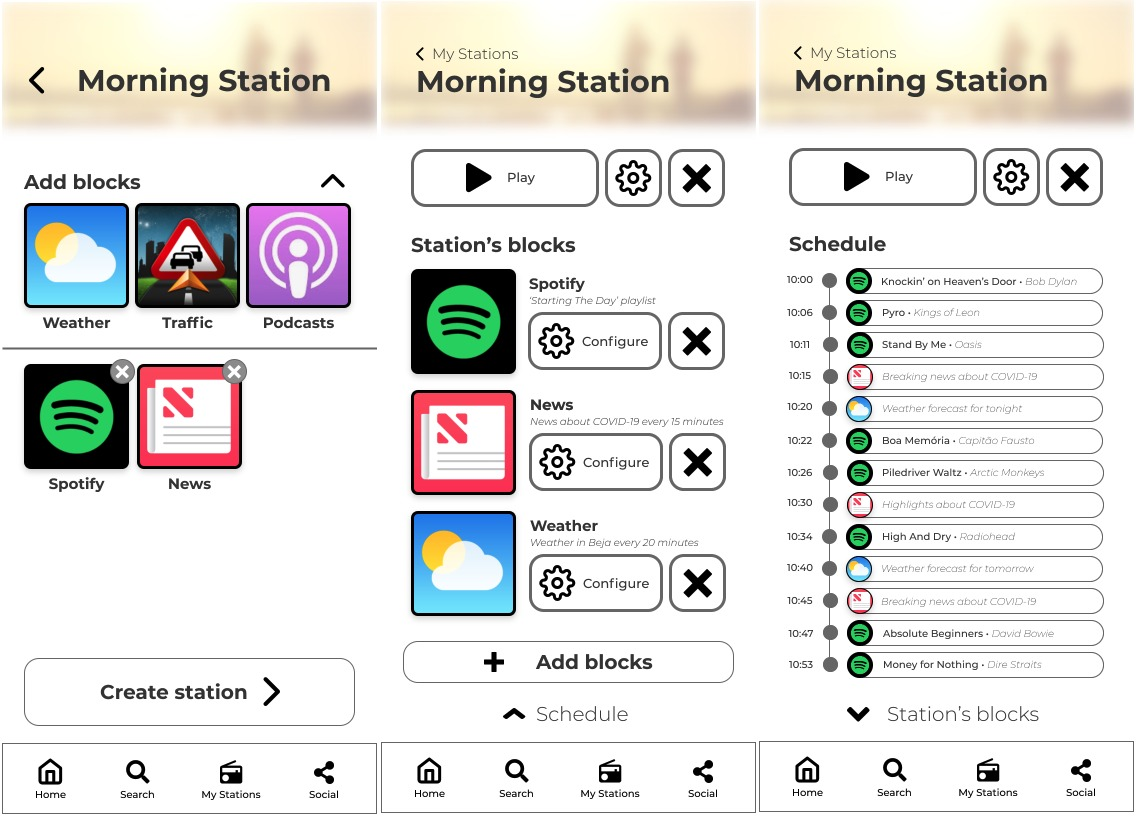
\includegraphics[width=\columnwidth]{./Images/prototype.jpg}
    \caption{Screenshots of the developed Sterio medium fidelity prototype.}
    \label{fig:persona}
\end{figure}

Given the before-mentioned COVID-19 pandemic we faced during the development of this study, the diffusion of the prototype was conducted using the WhatsApp social network, complying with social distancing restrictions. Groups with 4 users were created (larger numbers were avoided in order to make the discussion easier). In total, 7 groups of 4 people were created, totaling 28 participants in this study. 15 users were of ages ranging from 18 to 25, whilst the remaining 13 were of ages ranging from 26 to 62. The participating users are reported in table ~\ref{tab:users}.

Since the discussion of this prototype was conducted using an instant messaging service, users were encouraged to share their opinions and engage in discussion with each other, providing useful feedback that should be taken into account when developing the final product. From the 28 users, 19 have participated in the need validation activity of the speed dating method, thus an introduction to the general concept of the platform wasn't necessary. The remaining 9 users were introduced to the main abstract of the project and were asked to sign a virtual consent form. Users were informed that the displayed interface was created for demonstration purposes only, and that it didn't match the final product, shifting away their attention to the general concept of the system and not its usability.

The middle-fidelity prototype was created using three main tools: Adobe XD, Audacity, and macOS Text To Speech voices. 

Adobe XD was used for the development of the dummy interface. This platform allows playback of an audio file, which was convenient to showcase the final concept of the platform. The app also allows an easy sharing of the prototype, guiding them through its available options. 

Audacity was used to create the radio station audible file. The app allowed the editing of the audio file, making easy to expose how a created radio station would sound by gathered all the various audible elements (text-to-speech, music, and transitions). 

Finally, macOS' built-in text-to-speech software was used to synthesize into speech the content that the dummy user would provide (in this case, news and weather information). We opted for this solution since the operating system has a built-in European Portuguese voice (Catarina) that sounded very reliable and natural, making the development of the prototype a simpler task.

Corroborating with the first step of the method, the received feedback was very positive. All users clearly understood the main concept of the platform. Some of them mentioned that, in a first stage, they didn't understand the conceptualization on paper, but the prototype did enlighten them by showing in a visual and practical way how the platform would work.

Regarding the text-to-speech usage on the prototype, the feedback received was better than expected. The majority of users thought that the text-to-speech voice mimicking a radio host was more natural than what they were expecting. When asked if they felt a human element, and/or a connection with them in a similar way that traditional radio stations provide, all users replied affirmatively. In particular, older users accepted the text-to-speech functionalities quite well, with some mentioning that their original perception of this software (such as GPS turn-by-turn instructions) was out-blown with the use of this particular voice. Some younger users noted that the pronunciation of a small set of words was not clear or sounded unnatural, mainly new words (such as 'COVID-19') or foreignisms. Nevertheless, most of them noted that the advantages of using this technology outweigh the drawbacks.

Most users noted that they would use the platform on a daily basis, while others said it would be particularly interesting to use on specific occasions (such as driving or cooking). Some suggestions for future implementation on the system were also given by the users, such as the possibility for selecting their desired voice in their language, or a ‘quick station’ feature for the times when they would like to listen to a personalized radio based on their taste without a higher level of customization.